
\newpage
1kb MENOS DE UN SEGUNDO

1mb MENOS DE UN SEGUNDO

10 mb MENOS DE UN SEGUNDO
100 mb 2 SEGUNDOS +-1

1gb 32 SEGUNDOS 23 SEGUNODOS, 28 SEGUNDOS +- 5

2gb 42 SEGUNDOS, 40 SEGUNDOS 1MIN 2SEGUNDOS +-20

5gb3MIN 11SEC ,2 min 20 sec,3min 2 sec +- 40
10 gb 7min  32 sec+-2 min 


HAY QUE TENER EN CUENTA EL TAMAÑO DEL POOL
\newpage








------------------------

1gb 28 SEGUNDOS +- 5

1/2gb 18 sec 45 sec 1 min 42 sec

1/4gb 55sec  46 sec 49sec

1/8gb 25 sec 42 sec 1min6sec 30 sec 1min36sec 22sec 1min2sec 33sec
 
1/16gb 33sec 39 sec 46sec 27sec 26sec


--------------------------------------------



ahora viene algo complejo que no se que graficas, quiero ver como afecta los niveles de compresion, lzo y gzip del 1 al 9, 





archivos 42 MB

lzo COMPRESION
  Elapsed time:           5 secs
  Priority:               10
  FD Files Written:       2,994
  SD Files Written:       2,994
  FD Bytes Written:       35,940,395 (35.94 MB)
  SD Bytes Written:       36,345,644 (36.34 MB)
  Rate:                   7188.1 KB/s
  Software Compression:   18.4% 1.2:1
  
GZIP1 
  Elapsed time:           5 secs
  Priority:               10
  FD Files Written:       2,994
  SD Files Written:       2,994
  FD Bytes Written:       33,851,403 (33.85 MB)
  SD Bytes Written:       34,256,652 (34.25 MB)
  Rate:                   6770.3 KB/s
  Software Compression:   23.1% 1.3:1
  Comm Line Compression:  None

  
GZIP2
  Elapsed time:           6 secs
  Priority:               10
  FD Files Written:       2,994
  SD Files Written:       2,994
  FD Bytes Written:       33,785,906 (33.78 MB)
  SD Bytes Written:       34,191,155 (34.19 MB)
  Rate:                   5631.0 KB/s
  Software Compression:   23.3% 1.3:1

GZIP3
  Elapsed time:           6 secs
  Priority:               10
  FD Files Written:       2,994
  SD Files Written:       2,994
  FD Bytes Written:       33,746,172 (33.74 MB)
  SD Bytes Written:       34,151,421 (34.15 MB)
  Rate:                   5624.4 KB/s
  Software Compression:   23.3% 1.3:1
  
GZIP4
  Elapsed time:           5 secs
  Priority:               10
  FD Files Written:       2,994
  SD Files Written:       2,994
  FD Bytes Written:       33,650,630 (33.65 MB)
  SD Bytes Written:       34,055,879 (34.05 MB)
  Rate:                   6730.1 KB/s
  Software Compression:   23.6% 1.3:1

GZIP5
  Elapsed time:           5 secs
  Priority:               10
  FD Files Written:       2,994
  SD Files Written:       2,994
  FD Bytes Written:       33,600,422 (33.60 MB)
  SD Bytes Written:       34,005,671 (34.00 MB)
  Rate:                   6720.1 KB/s
  Software Compression:   23.7% 1.3:1
  
GZIP6
  Elapsed time:           5 secs
  Priority:               10
  FD Files Written:       2,994
  SD Files Written:       2,994
  FD Bytes Written:       33,563,434 (33.56 MB)
  SD Bytes Written:       33,968,683 (33.96 MB)
  Rate:                   6712.7 KB/s
  Software Compression:   23.8% 1.3:1

GZIP7
  Elapsed time:           5 secs
  Priority:               10
  FD Files Written:       2,994
  SD Files Written:       2,994
  FD Bytes Written:       33,554,589 (33.55 MB)
  SD Bytes Written:       33,959,838 (33.95 MB)
  Rate:                   6710.9 KB/s
  Software Compression:   23.8% 1.3:1

GZIP8
  Elapsed time:           5 secs
  Priority:               10
  FD Files Written:       2,994
  SD Files Written:       2,994
  FD Bytes Written:       33,539,830 (33.53 MB)
  SD Bytes Written:       33,945,079 (33.94 MB)
  Rate:                   6708.0 KB/s
  Software Compression:   23.8% 1.3:1
GZIP9
  Elapsed time:           5 secs
  Priority:               10
  FD Files Written:       2,994
  SD Files Written:       2,994
  FD Bytes Written:       33,538,224 (33.53 MB)
  SD Bytes Written:       33,943,473 (33.94 MB)
  Rate:                   6707.6 KB/s
  Software Compression:   23.8% 1.3:1



  
archivos 3.079gb

lzo COMPRESION
  Elapsed time:           2 mins 4 secs
  Priority:               10
  FD Files Written:       3,029
  SD Files Written:       3,029
  FD Bytes Written:       2,365,294,716 (2.365 GB)
  SD Bytes Written:       2,365,704,564 (2.365 GB)
  Rate:                   19075.0 KB/s
  Software Compression:   30.2% 1.4:1

GZIP1
  Elapsed time:           2 mins 38 secs
  Priority:               10
  FD Files Written:       3,029
  SD Files Written:       3,029
  FD Bytes Written:       2,311,167,033 (2.311 GB)
  SD Bytes Written:       2,311,576,881 (2.311 GB)
  Rate:                   14627.6 KB/s
  Software Compression:   31.8% 1.5:1
GZIP2
  Elapsed time:           2 mins 30 secs
  Priority:               10
  FD Files Written:       3,029
  SD Files Written:       3,029
  FD Bytes Written:       2,308,611,793 (2.308 GB)
  SD Bytes Written:       2,309,021,641 (2.309 GB)
  Rate:                   15390.7 KB/s
  Software Compression:   31.9% 1.5:1

GZIP3
  Elapsed time:           2 mins 11 secs
  Priority:               10
  FD Files Written:       3,029
  SD Files Written:       3,029
  FD Bytes Written:       2,303,626,262 (2.303 GB)
  SD Bytes Written:       2,304,036,110 (2.304 GB)
  Rate:                   17584.9 KB/s
  Software Compression:   32.0% 1.5:1
GZIP4
  Elapsed time:           2 mins 51 secs
  Priority:               10
  FD Files Written:       3,029
  SD Files Written:       3,029
  FD Bytes Written:       2,297,868,433 (2.297 GB)
  SD Bytes Written:       2,298,278,281 (2.298 GB)
  Rate:                   13437.8 KB/s
  Software Compression:   32.2% 1.5:1
GZIP5
  Elapsed time:           3 mins 
  Priority:               10
  FD Files Written:       3,029
  SD Files Written:       3,029
  FD Bytes Written:       2,291,542,206 (2.291 GB)
  SD Bytes Written:       2,291,952,054 (2.291 GB)
  Rate:                   12730.8 KB/s
  Software Compression:   32.4% 1.5:1

GZIP6
  Elapsed time:           2 mins 44 secs
  Priority:               10
  FD Files Written:       3,029
  SD Files Written:       3,029
  FD Bytes Written:       2,288,989,436 (2.288 GB)
  SD Bytes Written:       2,289,399,284 (2.289 GB)
  Rate:                   13957.3 KB/s
  Software Compression:   32.4% 1.5:1

GZIP7
  Elapsed time:           3 mins 1 sec
  Priority:               10
  FD Files Written:       3,029
  SD Files Written:       3,029
  FD Bytes Written:       2,286,067,346 (2.286 GB)
  SD Bytes Written:       2,286,477,194 (2.286 GB)
  Rate:                   12630.2 KB/s
  Software Compression:   32.5% 1.5:1

GZIP8
  Elapsed time:           3 mins 27 secs
  Priority:               10
  FD Files Written:       3,029
  SD Files Written:       3,029
  FD Bytes Written:       2,282,195,134 (2.282 GB)
  SD Bytes Written:       2,282,604,982 (2.282 GB)
  Rate:                   11025.1 KB/s
  Software Compression:   32.6% 1.5:1

GZIP9
  Elapsed time:           3 mins 52 secs
  Priority:               10
  FD Files Written:       3,029
  SD Files Written:       3,029
  FD Bytes Written:       2,282,104,121 (2.282 GB)
  SD Bytes Written:       2,282,513,969 (2.282 GB)
  Rate:                   13268.0 KB/s
  Software Compression:   32.6% 1.5:1



  %%%%%%%%%%%%%%%%%%%%%%%%%%%%%%%%%%%%%%%%
Restoring Files Can Be Slow
Restoring files is generally much slower than backing them up for several reasons. The first is that during a backup the tape is normally already positioned and Bacula only needs to write. On the other hand, because restoring files is done so rarely, Bacula keeps only the start file and block on the tape for the whole job rather than on a file by file basis which would use quite a lot of space in the catalog.

Bacula will forward space to the correct file mark on the tape for the Job, then forward space to the correct block, and finally sequentially read each record until it gets to the correct one(s) for the file or files you want to restore. Once the desired files are restored, Bacula will stop reading the tape.

Finally, instead of just reading a file for backup, during the restore, Bacula must create the file, and the operating system must allocate disk space for the file as Bacula is restoring it.

For all the above reasons the restore process is generally much slower than backing up (sometimes it takes three times as long).

restore

1kb 1sec

1mb 1sec

10mb 1sec

100mb 10sec 

1gb 48 secs

2gb 2 mins 36 secs

5gb 5 mins 45 secs

10gb  13 mins 30 secs

------------------------

1gb 48sec

1/2gb  21sec 

1/4gb  29sec

1/8gb  55 secs
 
1/16gb 1 min 13 secs


--------------------------------------------


estrategia gfs, granfather(monthly) dather(weekly) son(daily)
la granfather se toma siempre el 4 vierner del mes porque hay meses con 5 viernes
eponer esquema




Backup Continua (Continuous Data Protection, CDP):

Realiza backups de manera continua cada vez que se realiza un cambio en los datos.
Ventajas: Puntos de recuperación casi instantáneos.
Desventajas: Requiere un alto rendimiento de red y almacenamiento.

%%%%%%%%%%%%%%%%%%%%%%%%%%%%%%



\begin{figure}
    \centering
    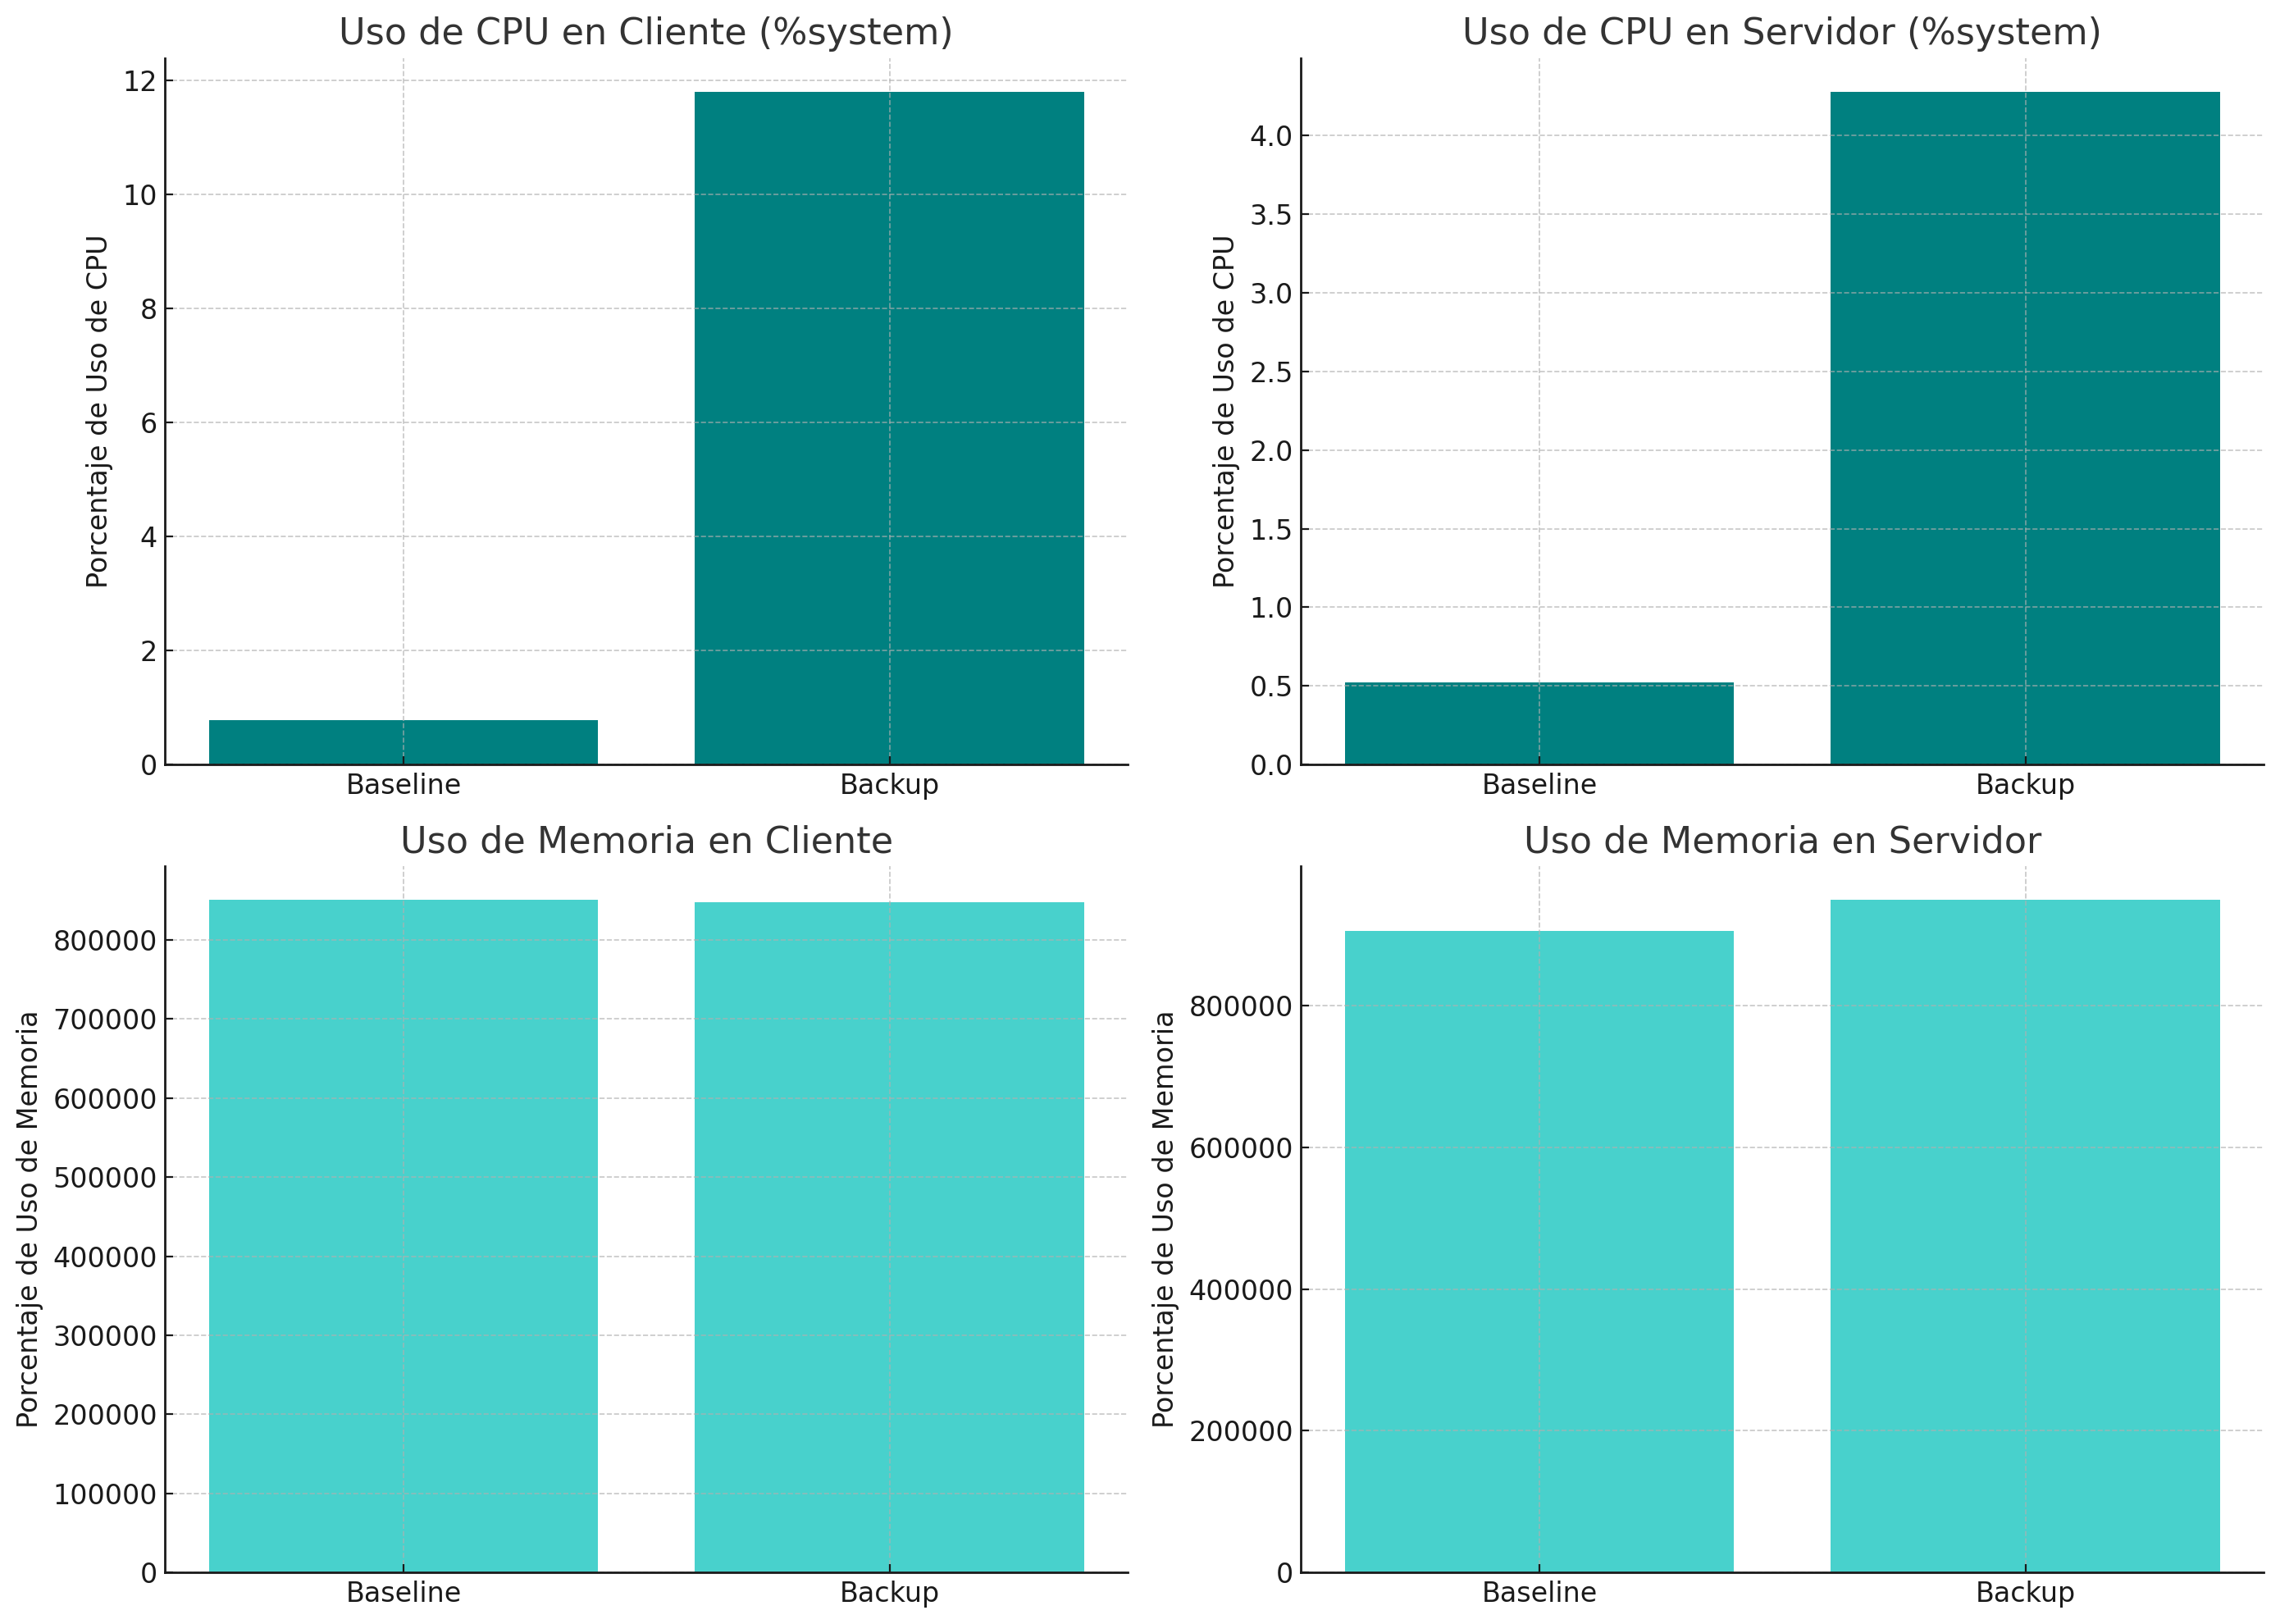
\includegraphics[width=0.5\linewidth]{uso_de_recursos.png}
    \caption{Enter Caption}
    \label{fig:enter-label}
\end{figure}